\subsection{Plutonium Redistribution}

As a consequence of restructuring, it became necessary to investigate the phenomenon of Plutonium redistribution. During restructuring, as observed, the formation of distinct zones occurs within the fuel element:

\begin{itemize}
    \item Central void
    \item Columnar grains (pores migrate, and mass is displaced outward)
    \item Equiaxed grains (caused by grain growth at high temperatures)
    \item As-fabricated (temperature is too low to cause changes)
\end{itemize}

These different zones are characterized by differences in density and, consequently, porosity. This is due to the densification of the fuel, reaching up to 98-99\% of TD.

Due to this phenomenon, the density variation results in a change in Plutonium concentration across the different zones of the fuel, which initially had a uniform concentration of 29\%. There is an enrichment of Plutonium in the central (columnar) zone, followed by an initial decrease reaching a minimum value, which corresponds to a depletion in the equiaxed zone. In the as-fabricated zone, the concentration stabilizes back to the initial value. The redistribution of Plutonium thus affects part of the fuel element and is a consequence of the high activation energy of Plutonium.

To evaluate how Plutonium redistribution varies following the phenomena of thermal expansion and fuel restructuring, we used the following formula, as provided in the handouts (Hot Effects Analysis, V):

\begin{equation}
    \frac{q'''(r)}{q_0} = \frac{c(r)}{c_0} = 1 + D \left\{ 
    \exp \left[ -2 \alpha \left( \frac{r - r^*}{R_\text{fo}} \right) \right] 
    - 2 \cdot \exp \left[ -\alpha \left( \frac{r - r^*}{R_\text{fo}} \right) \right]
    \right\}
\end{equation}
    

where:
\begin{itemize}
    \item $D = 0.01$ (from handouts),
    \item $\alpha$ is equal to 10 (from handouts),
    \item $r^*$ is an empirical constant set to $0.207 \cdot R_\text{fo}$, a value that ensures the conservation of Plutonium during redistribution,
    \item $C(r)$ is the radial Plutonium concentration [g/cm\(^3\)],
    \item $c_0$ is the initial Plutonium concentration.
\end{itemize}

Graphically, this result clearly illustrates all the phenomena associated with Plutonium redistribution.

\begin{figure}[H]
\centering
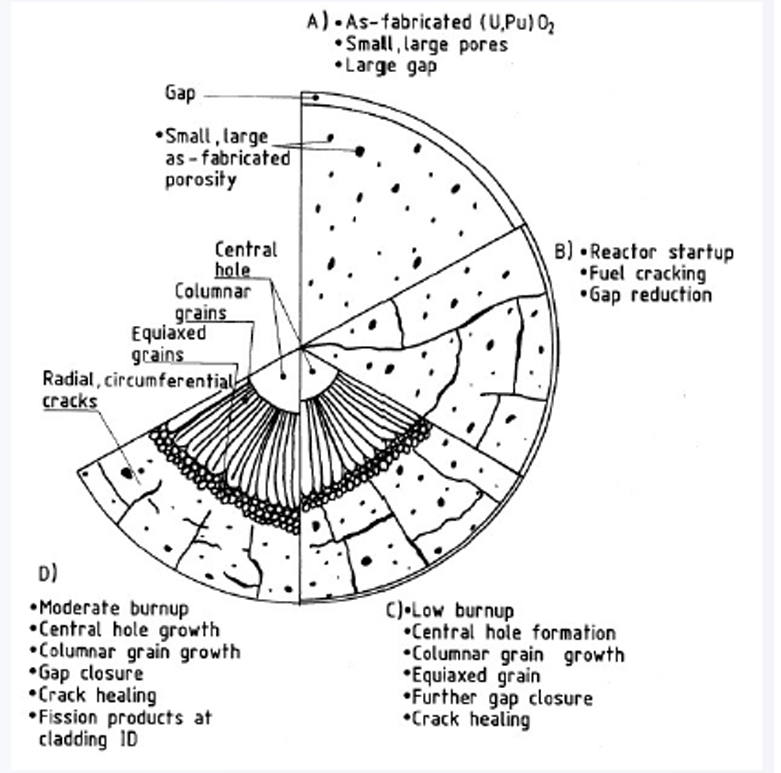
\includegraphics[width=0.8\textwidth]{Pu_redistributio_explaination.png}
\caption{Restructuring of fuel elements and formation of zones during irradiation.}
\label{fig:Redistribution_Structure}
\end{figure}

\begin{figure}[H]
\centering
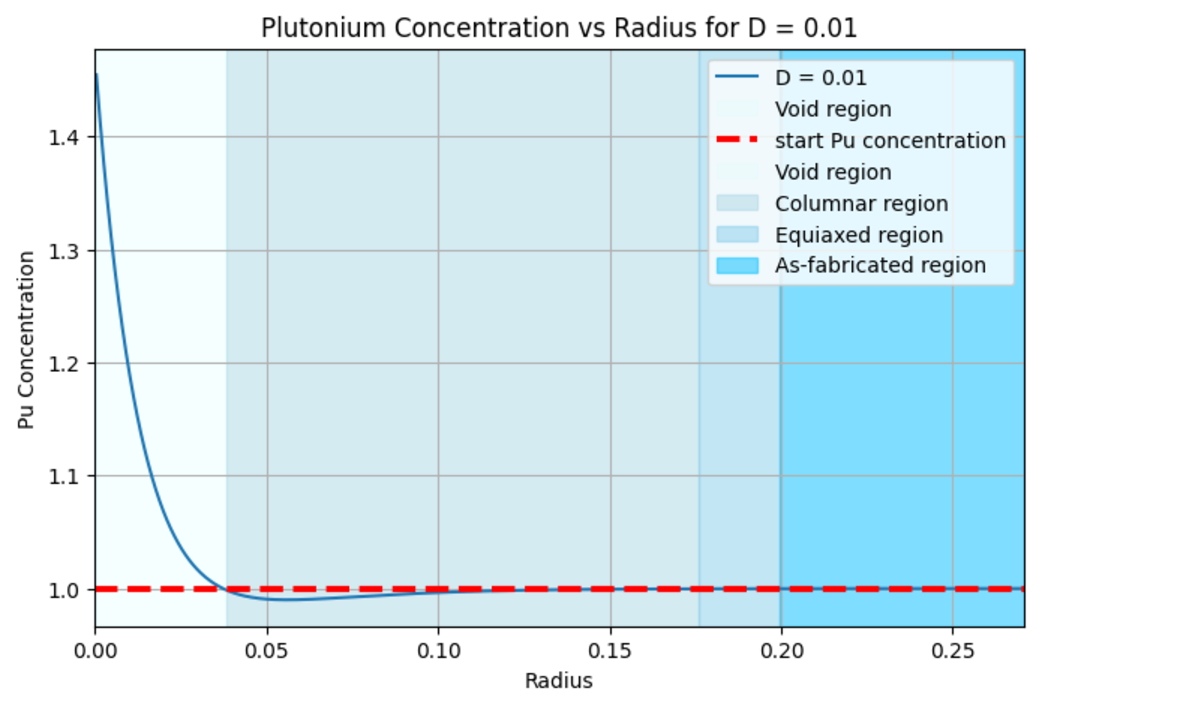
\includegraphics[width=0.8\textwidth]{Pu_redistribution_profile.png}
\caption{Radial distribution of Plutonium concentration (relative to starting concentration) within the fuel structure.}
\label{fig:Pu_Profile}
\end{figure}
